% Quantum Mechanics Mathematical Structure
% Comprehensive visual guide to the formalism used in quantum field theory

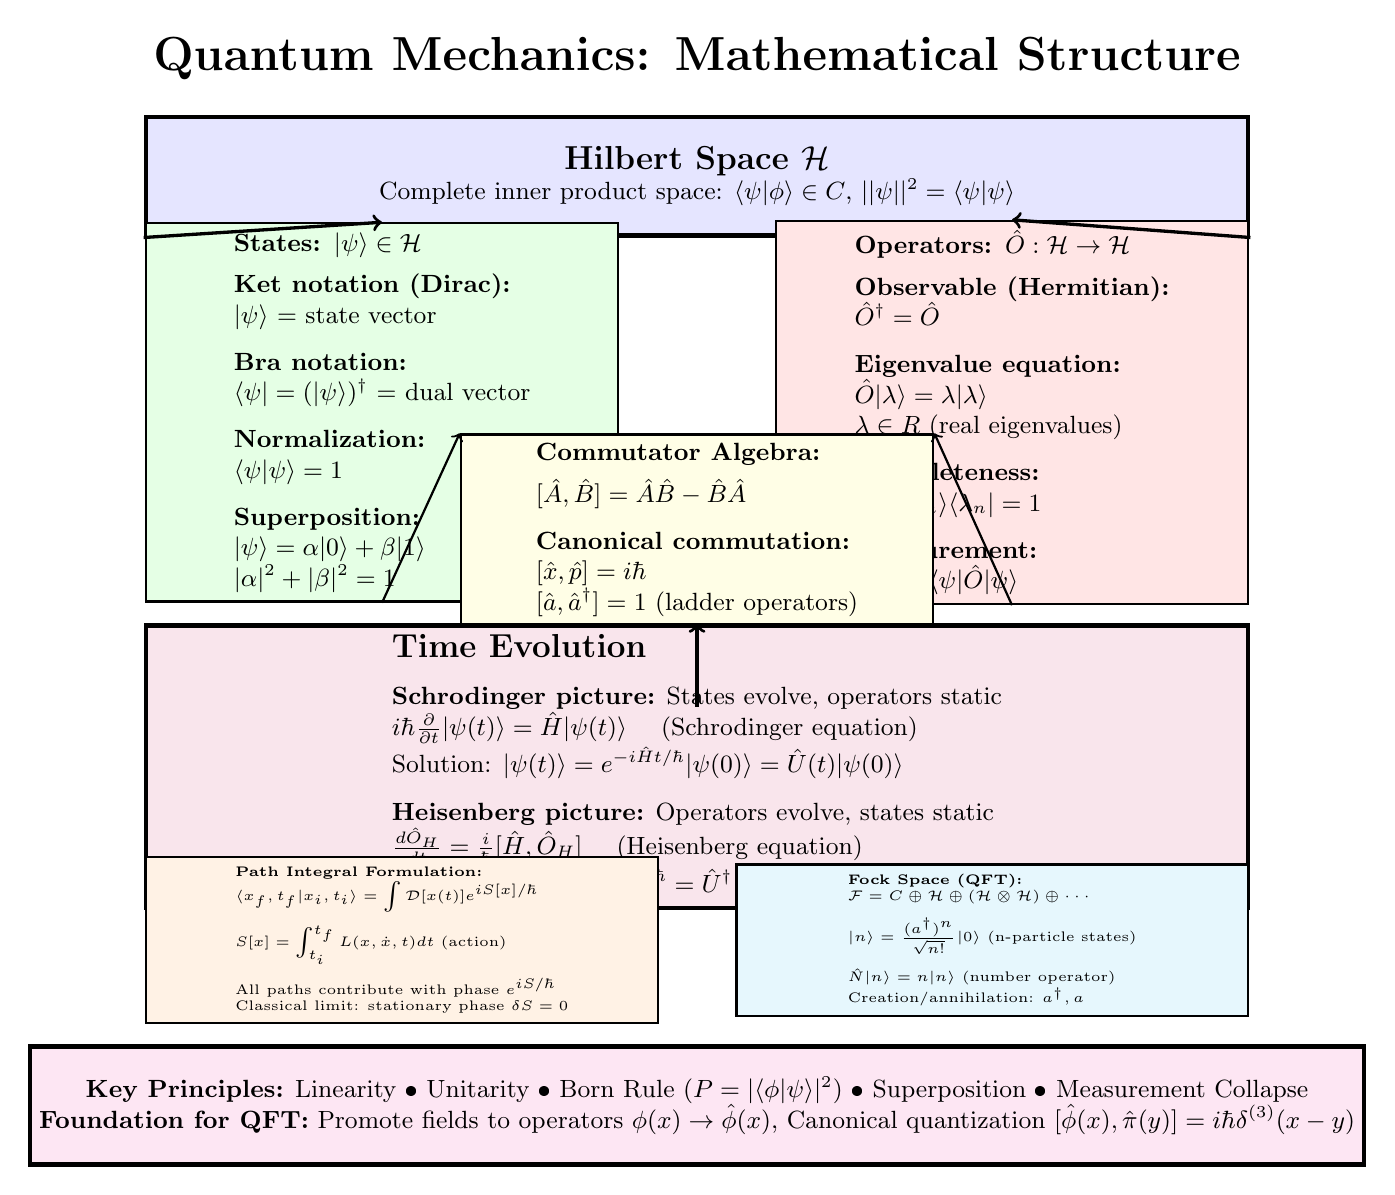
\begin{tikzpicture}[scale=1.0, every node/.style={font=\small}]

% Title
\node[font=\LARGE\bfseries] at (0,8) {Quantum Mechanics: Mathematical Structure};

% Hilbert Space (top level)
\node[draw, ultra thick, fill=blue!10, minimum width=14cm, minimum height=1.5cm, align=center] (hilbert) at (0,6.5) {
    \textbf{\large Hilbert Space $\mathcal{H}$}\\
    Complete inner product space: $\langle\psi|\phi\rangle \in \mathbb{C}$, $||\psi||^2 = \langle\psi|\psi\rangle$
};

% States (left branch)
\node[draw, thick, fill=green!10, minimum width=6cm, minimum height=3cm, align=left] (states) at (-4,3.5) {
    \textbf{States: $|\psi\rangle \in \mathcal{H}$}\\[4pt]
    \textbf{Ket notation (Dirac):}\\
    $|\psi\rangle$ = state vector\\[6pt]
    \textbf{Bra notation:}\\
    $\langle\psi| = (|\psi\rangle)^\dagger$ = dual vector\\[6pt]
    \textbf{Normalization:}\\
    $\langle\psi|\psi\rangle = 1$\\[6pt]
    \textbf{Superposition:}\\
    $|\psi\rangle = \alpha|0\rangle + \beta|1\rangle$\\
    $|\alpha|^2 + |\beta|^2 = 1$
};

% Operators (right branch)
\node[draw, thick, fill=red!10, minimum width=6cm, minimum height=3cm, align=left] (ops) at (4,3.5) {
    \textbf{Operators: $\hat{O}: \mathcal{H} \to \mathcal{H}$}\\[4pt]
    \textbf{Observable (Hermitian):}\\
    $\hat{O}^\dagger = \hat{O}$\\[6pt]
    \textbf{Eigenvalue equation:}\\
    $\hat{O}|\lambda\rangle = \lambda|\lambda\rangle$\\
    $\lambda \in \mathbb{R}$ (real eigenvalues)\\[6pt]
    \textbf{Completeness:}\\
    $\sum_n |\lambda_n\rangle\langle\lambda_n| = \mathbb{1}$\\[6pt]
    \textbf{Measurement:}\\
    $\langle\hat{O}\rangle = \langle\psi|\hat{O}|\psi\rangle$
};

% Arrows connecting
\draw[->, very thick] (hilbert.south west) -- (states.north);
\draw[->, very thick] (hilbert.south east) -- (ops.north);

% Commutator algebra (middle)
\node[draw, thick, fill=yellow!10, minimum width=6cm, minimum height=2cm, align=left] (comm) at (0,1.5) {
    \textbf{Commutator Algebra:}\\[4pt]
    $[\hat{A}, \hat{B}] = \hat{A}\hat{B} - \hat{B}\hat{A}$\\[6pt]
    \textbf{Canonical commutation:}\\
    $[\hat{x}, \hat{p}] = i\hbar$\\
    $[\hat{a}, \hat{a}^\dagger] = 1$ (ladder operators)\\[6pt]
    \textbf{Uncertainty principle:}\\
    $\Delta A \cdot \Delta B \geq \frac{1}{2}|\langle[\hat{A},\hat{B}]\rangle|$
};

% Arrows from states and operators to commutator
\draw[->, thick] (states.south) -- (comm.north west);
\draw[->, thick] (ops.south) -- (comm.north east);

% Time evolution (bottom level)
\node[draw, ultra thick, fill=purple!10, minimum width=14cm, minimum height=2.5cm, align=left] (time) at (0,-1) {
    \textbf{\large Time Evolution}\\[6pt]
    \textbf{Schrodinger picture:} States evolve, operators static\\
    $i\hbar\frac{\partial}{\partial t}|\psi(t)\rangle = \hat{H}|\psi(t)\rangle$ \quad (Schrodinger equation)\\
    Solution: $|\psi(t)\rangle = e^{-i\hat{H}t/\hbar}|\psi(0)\rangle = \hat{U}(t)|\psi(0)\rangle$\\[6pt]
    \textbf{Heisenberg picture:} Operators evolve, states static\\
    $\frac{d\hat{O}_H}{dt} = \frac{i}{\hbar}[\hat{H}, \hat{O}_H]$ \quad (Heisenberg equation)\\
    $\hat{O}_H(t) = e^{i\hat{H}t/\hbar}\hat{O}e^{-i\hat{H}t/\hbar} = \hat{U}^\dagger(t)\hat{O}\hat{U}(t)$
};

% Arrow from commutator to time evolution
\draw[->, very thick] (comm.south) -- (time.north);

% Path integral (bottom box)
\node[draw, thick, fill=orange!10, minimum width=6.5cm, minimum height=1.8cm, align=left, font=\tiny] (path) at (-3.75,-3.2) {
    \textbf{Path Integral Formulation:}\\
    $\langle x_f, t_f | x_i, t_i \rangle = \int \mathcal{D}[x(t)] e^{iS[x]/\hbar}$\\[4pt]
    $S[x] = \int_{t_i}^{t_f} L(x, \dot{x}, t) dt$ (action)\\[4pt]
    All paths contribute with phase $e^{iS/\hbar}$\\
    Classical limit: stationary phase $\delta S = 0$
};

% Fock space (bottom right box)
\node[draw, thick, fill=cyan!10, minimum width=6.5cm, minimum height=1.8cm, align=left, font=\tiny] (fock) at (3.75,-3.2) {
    \textbf{Fock Space (QFT):}\\
    $\mathcal{F} = \mathbb{C} \oplus \mathcal{H} \oplus (\mathcal{H} \otimes \mathcal{H}) \oplus \cdots$\\[4pt]
    $|n\rangle = \frac{(a^\dagger)^n}{\sqrt{n!}}|0\rangle$ (n-particle states)\\[4pt]
    $\hat{N}|n\rangle = n|n\rangle$ (number operator)\\
    Creation/annihilation: $a^\dagger, a$
};

% Key principles box
\node[draw, ultra thick, fill=magenta!10, minimum width=14cm, minimum height=1.5cm, align=center] (key) at (0,-5.3) {
    \textbf{Key Principles:} Linearity • Unitarity • Born Rule ($P = |\langle\phi|\psi\rangle|^2$) • Superposition • Measurement Collapse\\
    \textbf{Foundation for QFT:} Promote fields to operators $\phi(x) \to \hat{\phi}(x)$, Canonical quantization $[\hat{\phi}(x), \hat{\pi}(y)] = i\hbar\delta^{(3)}(x-y)$
};

\end{tikzpicture}
